\chapter{\ifenglish Background Knowledge and Theory\else ทฤษฎีที่เกี่ยวข้อง\fi}

การทำโครงงาน เริ่มต้นด้วยการศึกษาค้นคว้า ทฤษฎีที่เกี่ยวข้อง หรือ งานวิจัย/โครงงาน ที่เคยมีผู้นำเสนอไว้แล้ว ซึ่งเนื้อหาในบทนี้ก็จะเกี่ยวกับการอธิบายถึงสิ่งที่เกี่ยวข้องกับโครงงาน เพื่อให้ผู้อ่านเข้าใจเนื้อหาในบทถัดๆ ไปได้ง่ายขึ้น

\section{Ansible}
Ansible คือ Open Source Software ที่ทำหน้าที่เป็นเครื่องมือสำหรับการจัดการระบบ (IT automation) ที่ใช้เพื่อควบคุมและจัดการระบบต่างๆ บนเครือข่าย ใช้งานง่าย มีประสิทธิภาพ และมีความยืดหยุ่นสูง เขียนด้วยภาษา python และใช้ SSH (Secure Shell) ในการเชื่อมต่อกับระบบต่างๆ Ansible ทำงานโดยใช้ Playbook ซึ่งเป็นไฟล์ YAML (Yet Another Markup Language) ที่กำหนดชุดของ ta

รูปที่ \ref{fig:ansible_works} แสดงวิธีการทำงานของ Ansible
\begin{figure}
  \begin{center}
    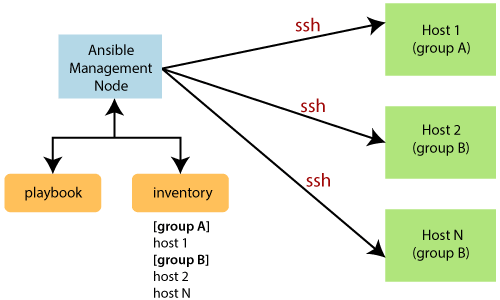
\includegraphics[scale=0.7]{ansible-works.png}
  \end{center}
  \caption[Poem]{วิธีการทำงานของ Ansible}
  \label{fig:ansible_works}
\end{figure}

\subsection{Inventory}
ไฟล์ที่ระบุรายการระบบปลายทางที่จะจัดการ
\subsection{Playbook}
ไฟล์ YAML ที่กำหนดชุดของ tasks ที่จะรันบนระบบปลายทาง
\subsection{Modules}
โมดูล python ที่ใช้เพื่อดำเนินการจัดการ tasks ต่างๆบนระบบปลายทาง
\subsection{Roles}
กลุ่มของ tasks ที่สามารถ reuse ได้

\section{AWX}
AWX เป็นเว็บอินเตอร์เฟสสำหรับ Ansible ช่วยให้ผู้ใช้สามารถจัดการ Ansible playbooks และ inventories ผ่านเว็บเบราว์เซอร์ AWX ทำให้การจัดการโครงสร้างพื้นฐาน IT ด้วย Ansible นั้นง่ายขึ้นและสะดวกยิ่งขึ้น โดยส่วนสำคัญของ AWX ได้แก่
\subsection{Dashboard}
สวัสดี

\subsection{Inventory}

Subsection 1 text

\subsection{Project}

Subsection 1 text

\subsection{Hosts}

Subsection 1 text

\subsection{Credential}

Subsection 1 text

\subsection{Templates}

Subsection 1 text

\subsection{Jobs}

Subsection 1 text

\subsubsection{Subsubsection 1 heading goes here}
Subsubsection 1 text

\subsubsection{Subsubsection 2 heading goes here}
Subsubsection 2 text

\section{Third section}
Section 3 text. The dielectric constant\index{dielectric constant}
at the air-metal interface determines
the resonance shift\index{resonance shift} as absorption or capture occurs
is shown in Equation~\eqref{eq:dielectric}:

\begin{equation}\label{eq:dielectric}
k_1=\frac{\omega}{c({1/\varepsilon_m + 1/\varepsilon_i})^{1/2}}=k_2=\frac{\omega
\sin(\theta)\varepsilon_\mathit{air}^{1/2}}{c}
\end{equation}

\noindent
where $\omega$ is the frequency of the plasmon, $c$ is the speed of
light, $\varepsilon_m$ is the dielectric constant of the metal,
$\varepsilon_i$ is the dielectric constant of neighboring insulator,
and $\varepsilon_\mathit{air}$ is the dielectric constant of air.

\section{About using figures in your report}

% define a command that produces some filler text, the lorem ipsum.
\newcommand{\loremipsum}{
  \textit{Lorem ipsum dolor sit amet, consectetur adipisicing elit, sed do
  eiusmod tempor incididunt ut labore et dolore magna aliqua. Ut enim ad
  minim veniam, quis nostrud exercitation ullamco laboris nisi ut
  aliquip ex ea commodo consequat. Duis aute irure dolor in
  reprehenderit in voluptate velit esse cillum dolore eu fugiat nulla
  pariatur. Excepteur sint occaecat cupidatat non proident, sunt in
  culpa qui officia deserunt mollit anim id est laborum.}\par}

\begin{figure}
  \centering

  \fbox{
     \parbox{.6\textwidth}{\loremipsum}
  }

  % To include an image in the figure, say myimage.pdf, you could use
  % the following code. Look up the documentation for the package
  % graphicx for more information.
  % \includegraphics[width=\textwidth]{myimage}

  \caption[Sample figure]{This figure is a sample containing \gls{lorem ipsum},
  showing you how you can include figures and glossary in your report.
  You can specify a shorter caption that will appear in the List of Figures.}
  \label{fig:sample-figure}
\end{figure}

Using \verb.\label. and \verb.\ref. commands allows us to refer to
figures easily. If we can refer to Figures
\ref{fig:walrus} and \ref{fig:sample-figure} by name in the {\LaTeX}
source code, then we will not need to update the code that refers to it
even if the placement or ordering of the figures changes.

\loremipsum\loremipsum

% This code demonstrates how to get a landscape table or figure. It
% uses the package lscape to turn everything but the page number into
% landscape orientation. Everything should be included within an
% \afterpage{ .... } to avoid causing a page break too early.
\afterpage{
  \begin{landscape}
  \begin{table}
    \caption{Sample landscape table}
    \label{tab:sample-table}

    \centering

    \begin{tabular}{c||c|c}
        Year & A & B \\
        \hline\hline
        1989 & 12 & 23 \\
        1990 & 4 & 9 \\
        1991 & 3 & 6 \\
    \end{tabular}
  \end{table}
  \end{landscape}
}

\loremipsum\loremipsum\loremipsum

\section{Overfull hbox}

When the \verb.semifinal. option is passed to the \verb.cpecmu. document class,
any line that is longer than the line width, i.e., an overfull hbox, will be
highlighted with a black solid rule:
\begin{center}
\begin{minipage}{2em}
juxtaposition
\end{minipage}
\end{center}

\section{\ifenglish%
\ifcpe CPE \else ISNE \fi knowledge used, applied, or integrated in this project
\else%
ความรู้ตามหลักสูตรซึ่งถูกนำมาใช้หรือบูรณาการในโครงงาน
\fi
}

อธิบายถึงความรู้ และแนวทางการนำความรู้ต่างๆ ที่ได้เรียนตามหลักสูตร ซึ่งถูกนำมาใช้ในโครงงาน

\section{\ifenglish%
Extracurricular knowledge used, applied, or integrated in this project
\else%
ความรู้นอกหลักสูตรซึ่งถูกนำมาใช้หรือบูรณาการในโครงงาน
\fi
}

อธิบายถึงความรู้ต่างๆ ที่เรียนรู้ด้วยตนเอง และแนวทางการนำความรู้เหล่านั้นมาใช้ในโครงงาน
